\begin{figure}
\centering
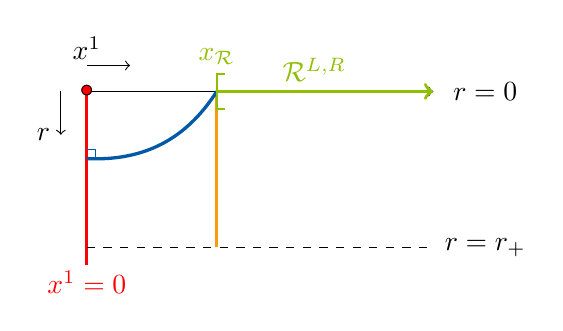
\begin{tikzpicture}[scale=1.1]
\draw[->] (0,2) to (2+2,2);
\draw[-,very thick,red] (0,2) to (0,0);

\draw[->] (0,2.3) to (0.5,2.3);
\node at (0,2.5) {$x^1$};

\draw[->] (-0.3,2) to (-0.3,1.5);
\node at (-0.5,1.5) {$r$};

\node at (0,-0.2) {\textcolor{red}{$x^1 = 0$}};

\draw[-,dashed] (0,0.2) to (2+2,0.2);

\node at (2+2.6,0.2) {$r = r_+$};
\node at (2+2.6,2) {$r = 0$};

\draw[-,yellow!20!orange,very thick] (1.5,2) to (1.5,0.2);
\draw[-,blue!30!teal,very thick] (1.5,2) to[bend left] (0,1.225);
\draw[-,blue!30!teal] (0.1,1.225) to (0.1,1.325) to (0,1.325);

\draw[->,very thick,black!25!lime] (1.5,2) to (4,2);
\node at (2.625,2.25) {\textcolor{black!25!lime}{$\mathcal{R}^{L,R}$}};

\draw[-,black!25!lime,thick] (1.6,2.2) to (1.5,2.2) to (1.5,1.8) to (1.6,1.8);
\node at (1.5,2.4) {\textcolor{black!25!lime}{$x_\mathcal{R}$}};

\node[color=red] at (0,2) {$\bullet$};
\node at (0,2) {$\circ$};
\end{tikzpicture}
\caption{The candidate RT surfaces in one of the exterior regions. The orange line entering the horizon is the Hartman-Maldacena surface, whereas the blue arc which ends perpendicularly on the brane is the island-producing exterior surface.}
\label{figs:candidateSurfaces}
\end{figure}